\tikzset{every picture/.style={line width=0.75pt}} %set default line width to 0.75pt        

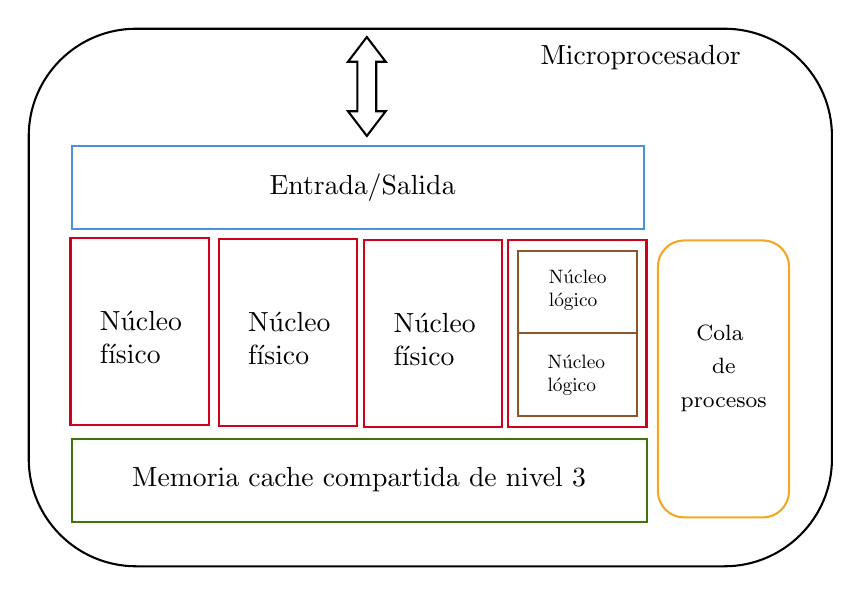
\begin{tikzpicture}[x=0.75pt,y=0.75pt,yscale=-1,xscale=1]
%uncomment if require: \path (0,300); %set diagram left start at 0, and has height of 300

%Shape: Rectangle [id:dp7451660985771589] 
\draw  [color={rgb, 255:red, 208; green, 2; blue, 27 }  ,draw opacity=1 ] (100.31,108) -- (166.81,108) -- (166.81,198.2) -- (100.31,198.2) -- cycle ;

%Shape: Rectangle [id:dp20887119442499946] 
\draw  [color={rgb, 255:red, 208; green, 2; blue, 27 }  ,draw opacity=1 ] (171.81,108.5) -- (238.31,108.5) -- (238.31,198.7) -- (171.81,198.7) -- cycle ;

%Shape: Rectangle [id:dp7286280016278224] 
\draw  [color={rgb, 255:red, 208; green, 2; blue, 27 }  ,draw opacity=1 ] (241.81,109) -- (308.31,109) -- (308.31,199.2) -- (241.81,199.2) -- cycle ;

%Shape: Rectangle [id:dp10536868660856769] 
\draw  [color={rgb, 255:red, 208; green, 2; blue, 27 }  ,draw opacity=1 ] (311.31,109) -- (377.81,109) -- (377.81,199.2) -- (311.31,199.2) -- cycle ;
%Shape: Rectangle [id:dp1826752439641639] 
\draw  [color={rgb, 255:red, 65; green, 117; blue, 5 }  ,draw opacity=1 ] (101.17,205.17) -- (378.06,205.17) -- (378.06,245.17) -- (101.17,245.17) -- cycle ;
%Rounded Rect [id:dp2234320479476144] 
\draw  [color={rgb, 255:red, 245; green, 166; blue, 35 }  ,draw opacity=1 ] (383.33,121.97) .. controls (383.33,114.99) and (388.99,109.33) .. (395.97,109.33) -- (433.87,109.33) .. controls (440.84,109.33) and (446.5,114.99) .. (446.5,121.97) -- (446.5,230.17) .. controls (446.5,237.14) and (440.84,242.8) .. (433.87,242.8) -- (395.97,242.8) .. controls (388.99,242.8) and (383.33,237.14) .. (383.33,230.17) -- cycle ;
%Shape: Rectangle [id:dp1417047542970684] 
\draw  [color={rgb, 255:red, 74; green, 144; blue, 226 }  ,draw opacity=1 ] (101,64) -- (376.5,64) -- (376.5,104) -- (101,104) -- cycle ;
%Shape: Rectangle [id:dp36104680527645483] 
\draw  [color={rgb, 255:red, 139; green, 87; blue, 42 }  ,draw opacity=1 ] (316,114.5) -- (373.25,114.5) -- (373.25,154.1) -- (316,154.1) -- cycle ;
%Shape: Rectangle [id:dp8737201655413631] 
\draw  [color={rgb, 255:red, 139; green, 87; blue, 42 }  ,draw opacity=1 ] (316,154.1) -- (373.25,154.1) -- (373.25,193.7) -- (316,193.7) -- cycle ;
%Rounded Rect [id:dp23562455979240182] 
\draw   (80.17,59.13) .. controls (80.17,30.52) and (103.36,7.33) .. (131.97,7.33) -- (415.37,7.33) .. controls (443.98,7.33) and (467.17,30.52) .. (467.17,59.13) -- (467.17,214.53) .. controls (467.17,243.14) and (443.98,266.33) .. (415.37,266.33) -- (131.97,266.33) .. controls (103.36,266.33) and (80.17,243.14) .. (80.17,214.53) -- cycle ;
%Up Down Arrow [id:dp8508564601094952] 
\draw   (234,23.25) -- (243.08,11.33) -- (252.17,23.25) -- (247.62,23.25) -- (247.62,47.08) -- (252.17,47.08) -- (243.08,59) -- (234,47.08) -- (238.54,47.08) -- (238.54,23.25) -- cycle ;

% Text Node
\draw (134.25,156) node  [align=left] {Núcleo\\ físico};
% Text Node
\draw (205.75,156.5) node  [align=left] {Núcleo\\ físico};
% Text Node
\draw (275.75,157) node  [align=left] {Núcleo\\ físico};
% Text Node
\draw (239.33,224.67) node  [align=left] {Memoria cache compartida de nivel 3};
% Text Node
\draw (415,171) node  [align=left] {{\footnotesize  \ \ Cola}\\{\footnotesize  \ \ \ \ de}\\{\footnotesize procesos}};
% Text Node
\draw (241,84) node  [align=left] {Entrada/Salida};
% Text Node
\draw (344.67,133.33) node [scale=0.7] [align=left] {Núcleo\\ lógico};
% Text Node
\draw (344,174.33) node [scale=0.7] [align=left] {Núcleo\\ lógico};
% Text Node
\draw (375,21) node  [align=left] {Microprocesador};


\end{tikzpicture}